\documentclass[11pt]{report}
\usepackage{float}
\usepackage{graphicx}
\usepackage{fullpage}

\newcommand{\define}[2] {
  \textbf{Definition: #1}
  \begin{center} #2
\end{center}
}

\begin{document}

\title{PMR lecture notes}
\maketitle

\chapter{Prerequisites}

\section{Joint probability distribution}
A joint probability distribution is the PD of two random variables. This must sum to 1 as the probability of some combination must be 1.

If there are only two random variables, this is known as a bivariate distribution. If there are more than two variables this is known as a multivariate distribution. 

\subsection{Conditioning}
We can use conditioning as a means of reducing a joint probability distribution. However, the reduced version results in an normalised distribution which no longer sums to 1. 

\chapter{Belief networks}

A Bayes(or belief) network is a directed acyclic graph (DAG) whose nodes represent random variables $X_1...X_n$. For each node, $X_i$ has a CPD $P(X_i  Par_G(x_i))$ which denotes dependency on it's parent.

\begin{figure}[H]
\centering
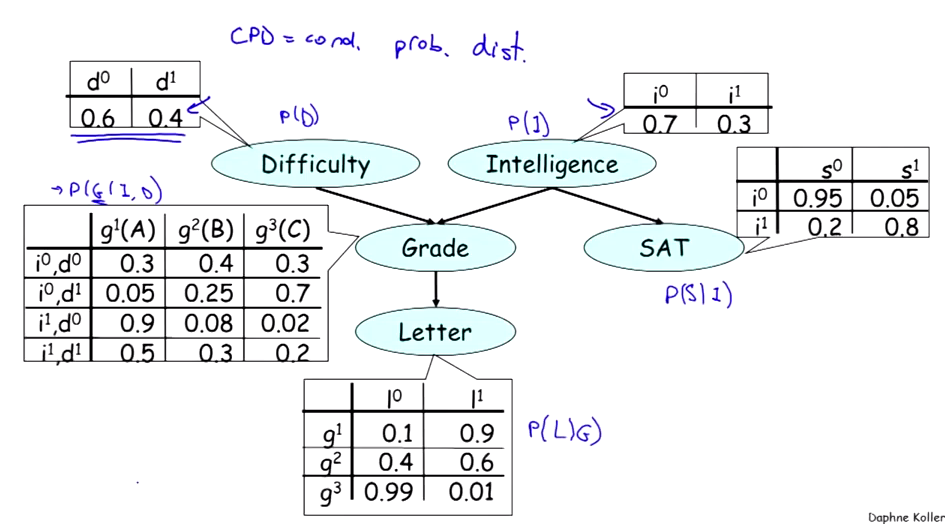
\includegraphics[width=90mm]{images/cpd_bayesnetwork.png}
\caption{Bayes network with CPD details}
\label{sensorymockup2}
\end{figure}

This is an example of a bayesian network. The probabilities are dependent on each other. \\

\define{Chain rule}{The chain rule takes all of the CPD's and multiplies them together}

\begin{figure}[H]
\centering
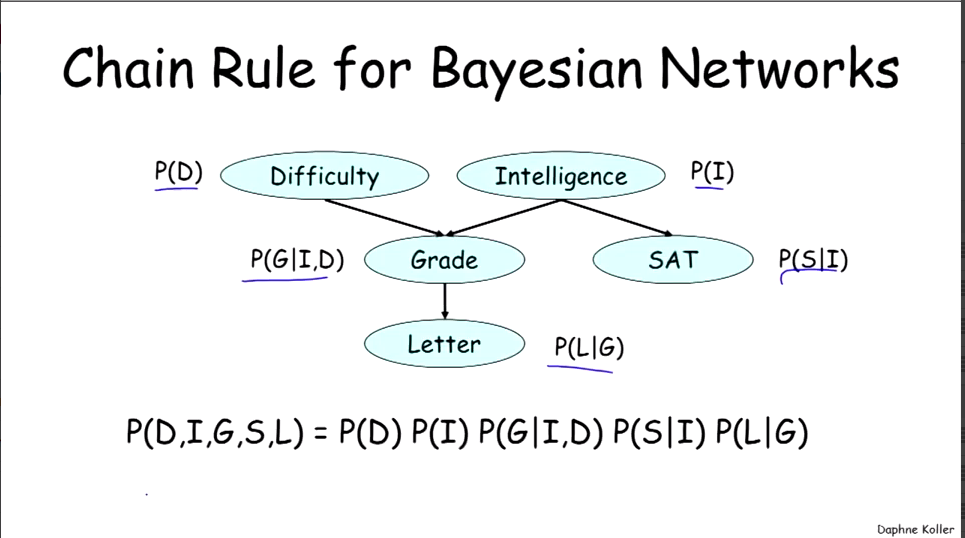
\includegraphics[width=90mm]{images/cpd_chainrule.png}
\caption{Bayes network with higher level details of CPDs}
\label{sensorymockup2}
\end{figure}



\chapter{Questions}

\section{Belief networks}
\subsection{Question 1}
What is $P(d^0, i^1, g^3, s^1, l^1)$?

Using the two images for information:

$i^1$ = 0.3 \\
$d^0$ = 0.6 \\
$l^1$ = 0.01 \\
$g^3$ = 0.02 \\
$s^1$ = 0.8 \\

And we can multiply these together to get the answer. 


\chapter{Glossary}
\define{CPD}{Conditional probability distribution}
\define{Conditioning}{When we set one of the probabilities values (we condition it) as a means of reducing the network. See Coursera(Week 1, Distributions)}


\end{document}